\documentclass[peerreview]{IEEEtran}
\usepackage{cite} % Tidies up citation numbers.
\usepackage{url} % Provides better formatting of URLs.
\usepackage[utf8]{inputenc} % Allows Turkish characters.
\usepackage{booktabs} % Allows the use of \toprule, \midrule and \bottomrule in tables for horizontal lines
\usepackage{graphicx}
\usepackage[colorlinks, linkcolor=blue]{hyperref}

\hyphenation{op-tical net-works semi-conduc-tor} % Corrects some bad hyphenation 



\begin{document}
%----------------------------------------------------------------------------------------
%	TITLE PAGE
%----------------------------------------------------------------------------------------

\begin{titlepage}
	
	\rule{\linewidth}{5pt}
	\raggedleft
	\fontsize{38pt}{50pt}\selectfont
    \textbf{\\Team Project\\}
    \fontsize{28pt}{60pt}\selectfont 
    for\\
    \fontsize{38pt}{60pt}\selectfont 
    \textbf{Submission 2\\}
	
	\vfill % Space between the title box and author information
	
	%------------------------------------------------
	%	Author name and information
	%------------------------------------------------
	
	\parbox[t]{0.93\textwidth}{ % Box to inset this section slightly
		\raggedleft % Right align the text
		\large % Increase the font size
		{\Large By Team 23-22}\\[4pt] % Extra space after name
		Zijun Li\_2272583\_zxl183\\
	}
	
\end{titlepage}

\newpage

{\Large\bf{Agile Estimation of Cards}}\\

\begin{itemize}
  {\bf\item To-do List(interface)  : 6 hours }
  \subitem It will involve creating an intuitive and visually appealing layout to effectively display the Todo items, Done items, and Details components.
  {\bf\item To-do List(Todo items) : 8 hours}
  \subitem It will include the implementation of the connection between Todo items and Done items, as well as the addition and removal of items. Effective data transfer with the database will also be a key consideration.
  {\bf\item To-do List(Done items) : 8 hours}
  \subitem It will include the implementation of the connection between Todo items and Done items, as well as the addition and removal of items. Effective data transfer with the database will also be a key consideration.
  {\bf\item To-do List(Details)    : 8 hours}
  \subitem The details of the chosen items, it also need to be linked to the database. 
  {\bf\item To-do List(Total)      : 36 hours(with extra 6 hours for checking)}
  \subitem  It includes all of the components listed above, as well as other functions related to the home page and checking.
\end{itemize}

\begin{figure}[!h]
  \centering
  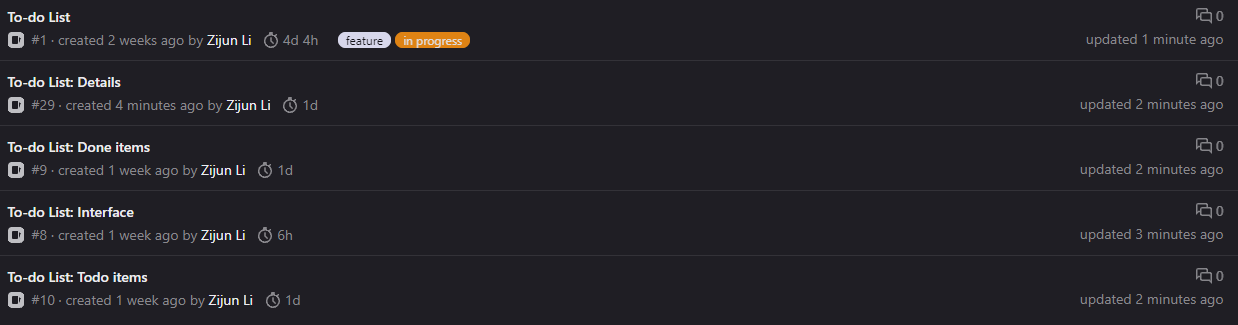
\includegraphics[width=1\columnwidth]{./images/Agile Estimation of Cards.png} 
  \label{fig_Agile}
\end{figure}

{\footnotesize It looks like gitlab treats 8 hours as 1 working day, so 7 hr becomes 7 hr, 8hr becomes 1 day, 9 hr becomes 1 day 1 hr etc.}

\newpage

{\Large\bf{Tech stack/CI}}\\

\begin{figure}[!h]
  \centering
  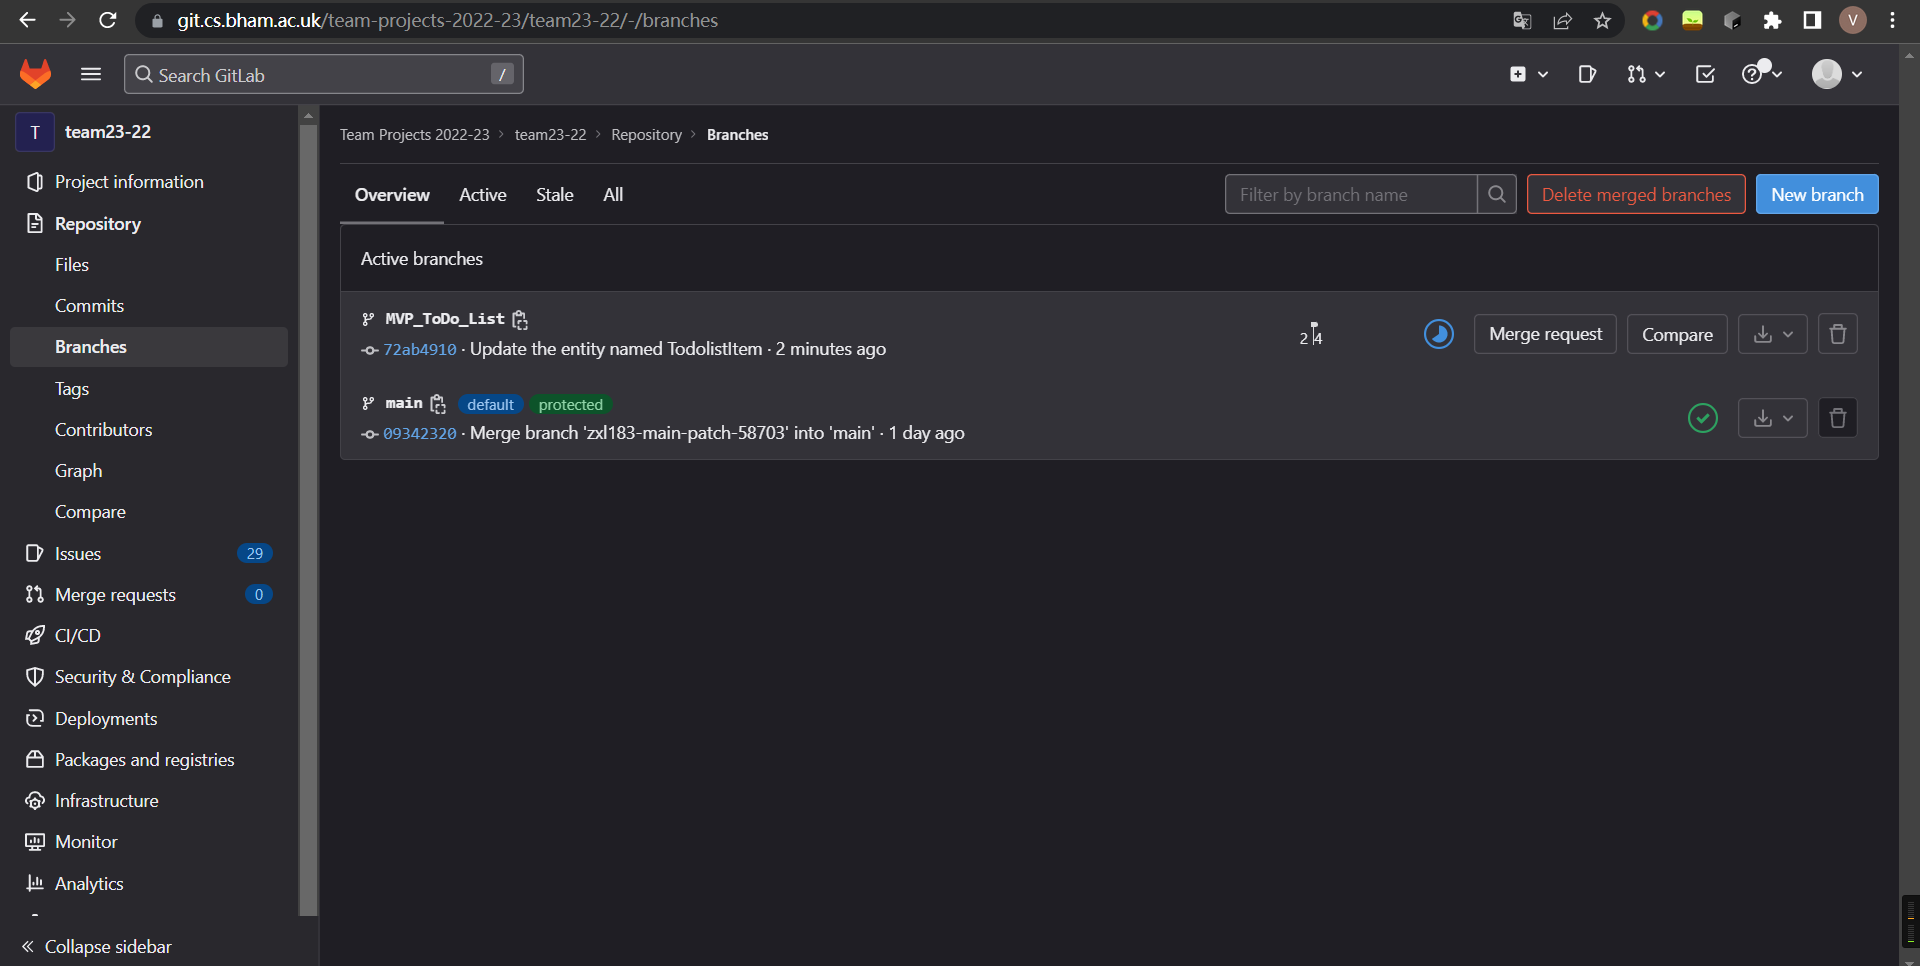
\includegraphics[width=1\columnwidth]{./images/MVP_1.png} 
  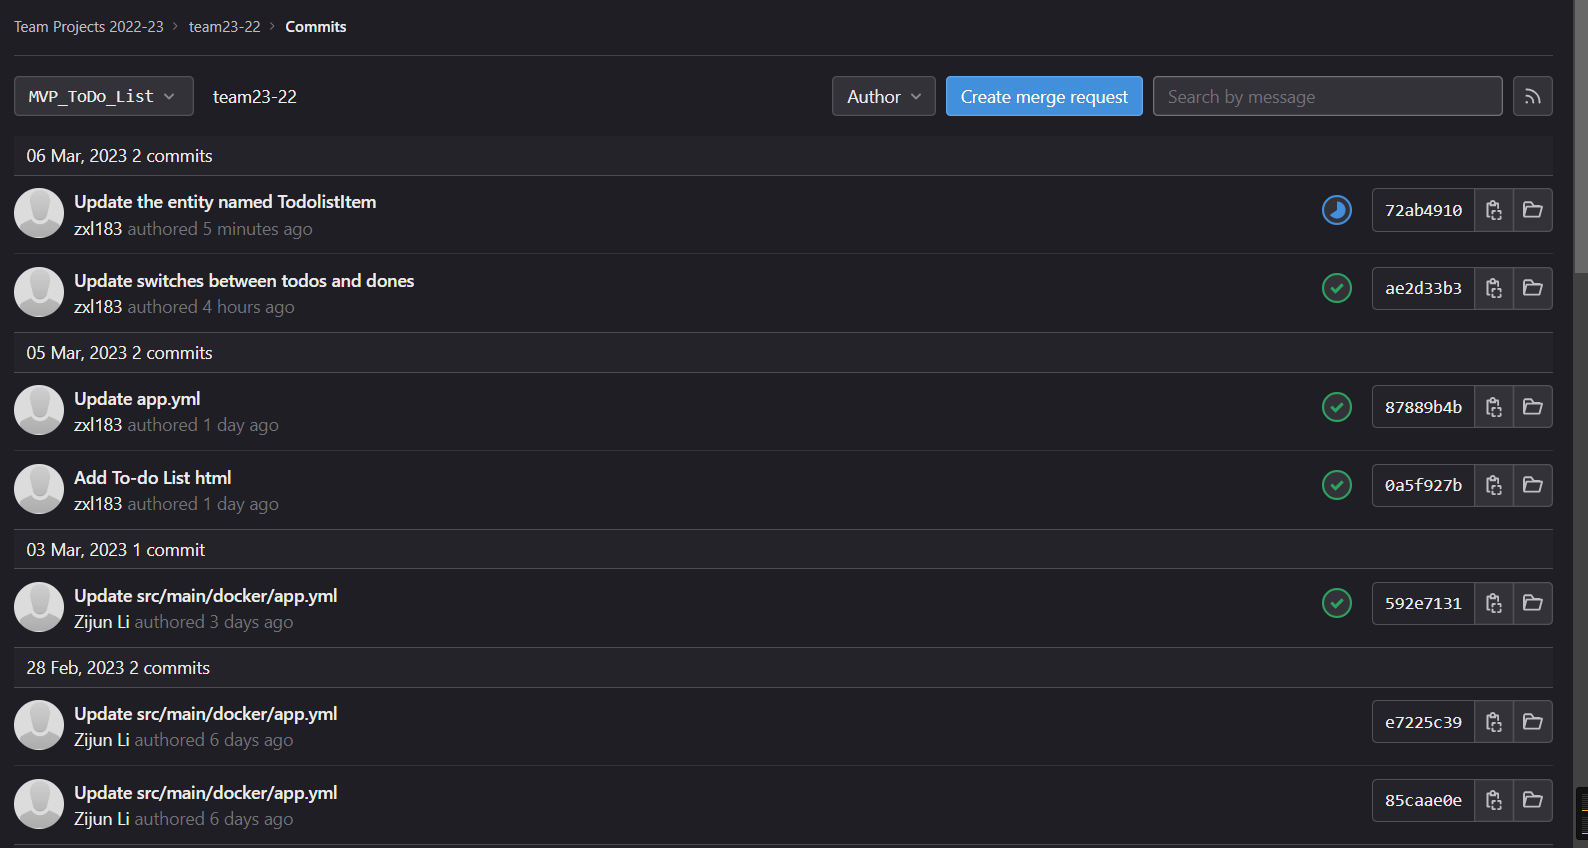
\includegraphics[width=1\columnwidth]{./images/MVP_2.png} 
  \label{fig_MVP_1}
\end{figure}

\newpage

\begin{figure}[!h]
  \centering
  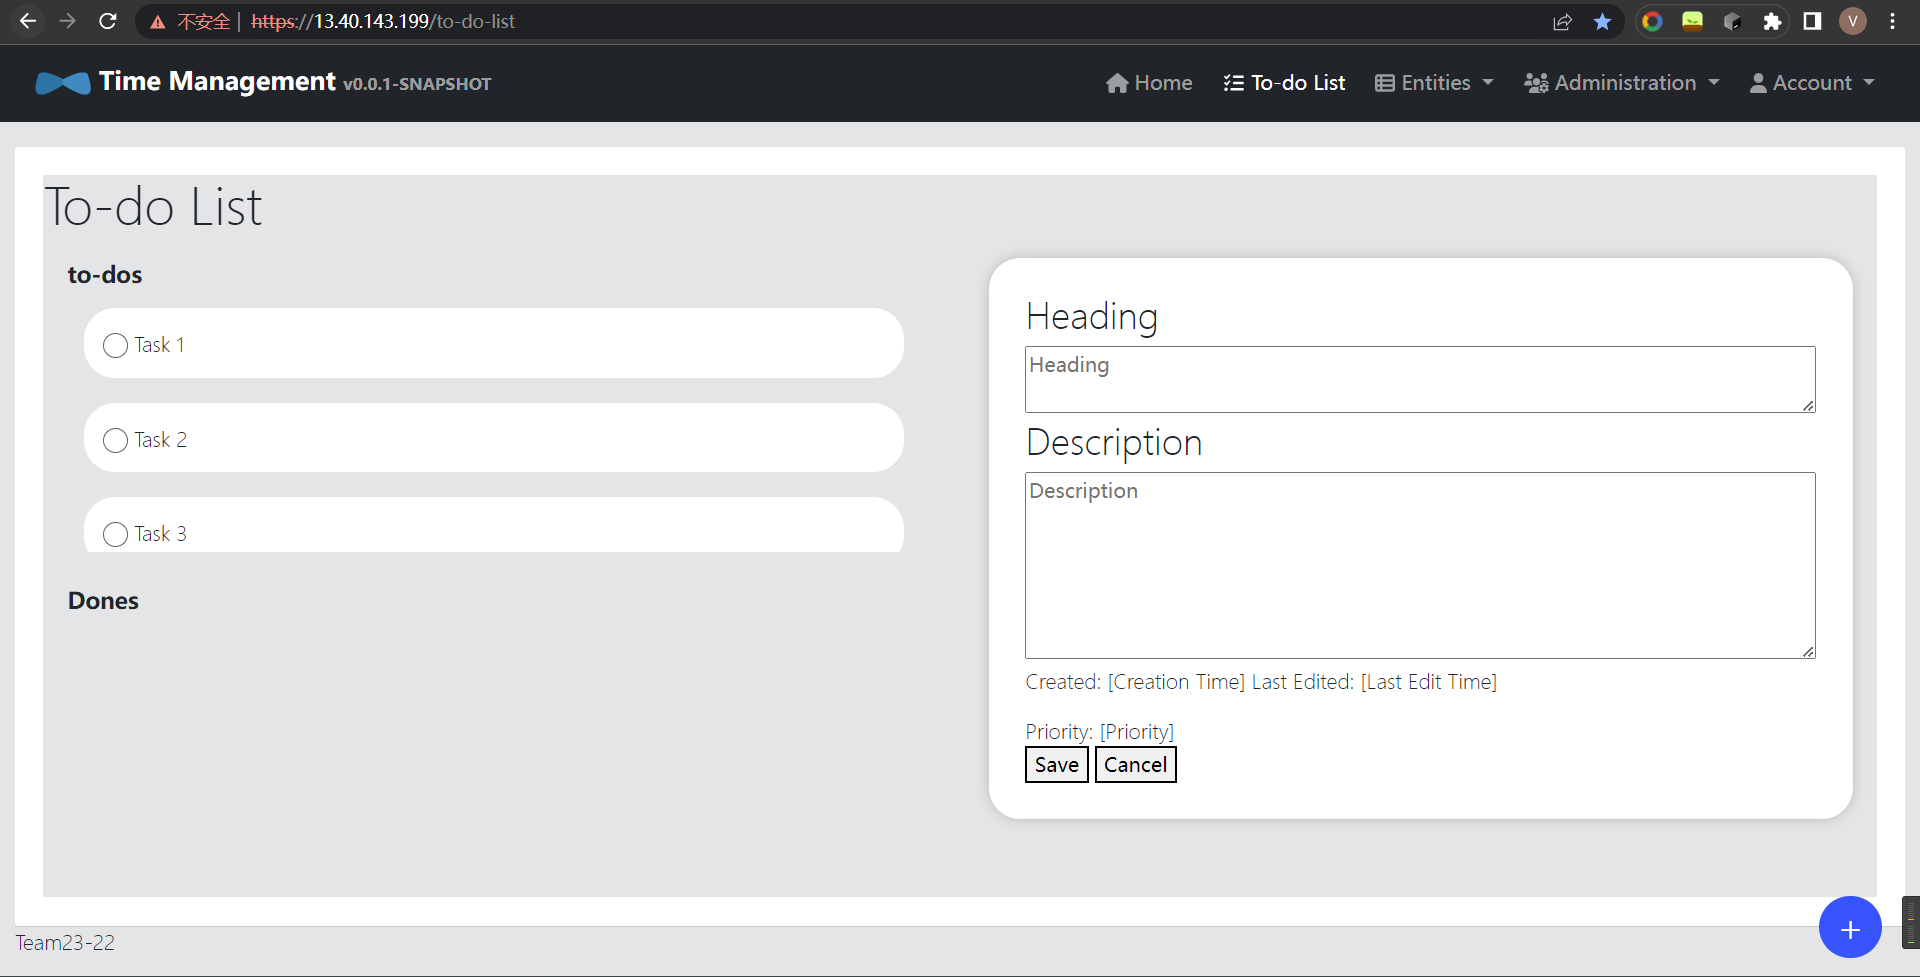
\includegraphics[width=1\columnwidth]{./images/MVP_3.png} 
  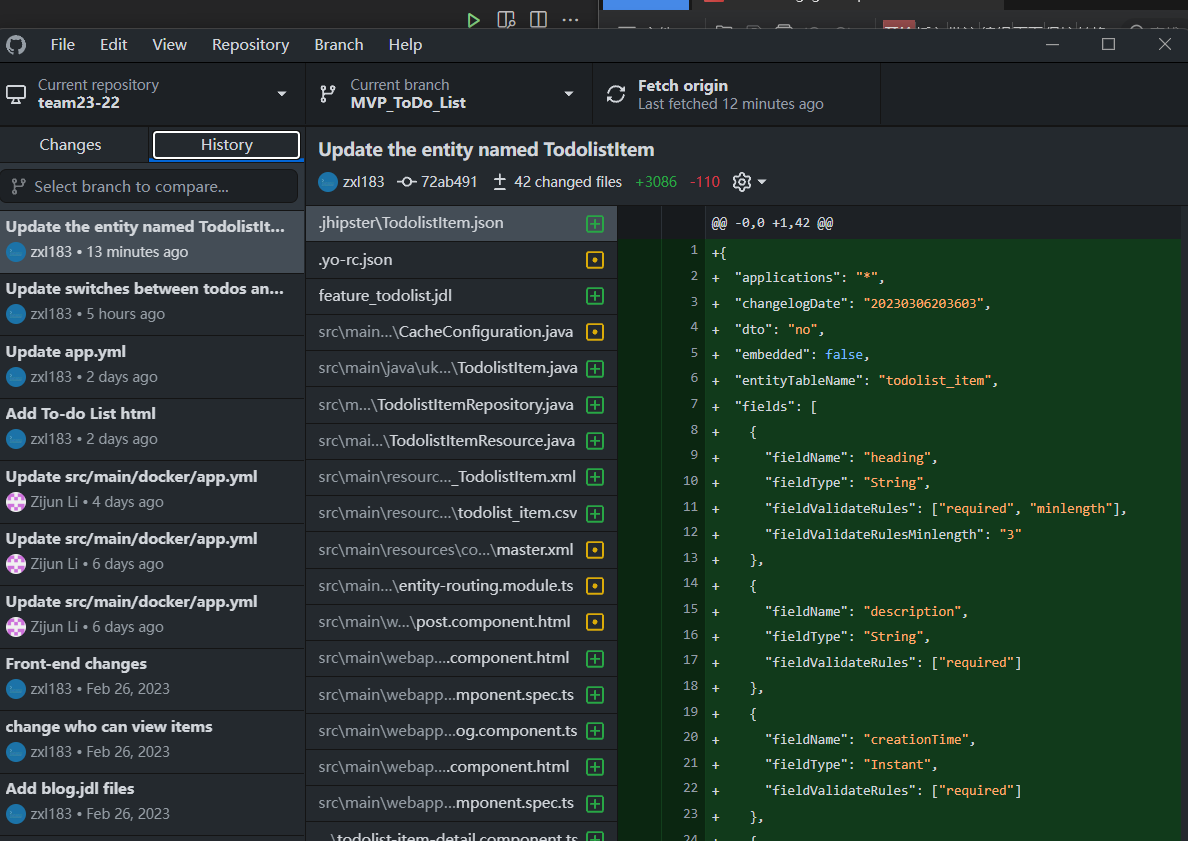
\includegraphics[width=1\columnwidth]{./images/MVP_4.png} 
  \label{fig_MVP_2}
\end{figure}



\newpage

\title{A Technical Report on Library/API Integration in Time Management Application.}
\IEEEpeerreviewmaketitle

\section{Introduction}
  In a Time Management Application, there are multiple layers that interact with each other, including the front-end, back-end, and database. These layers are composed of various features that require communication with one another to operate seamlessly. API integration plays a crucial role in facilitating this communication by providing a set of rules and protocols for data transfer and interaction. 

\section{Background}
  An API integration is the connection between two or more applications/features/layers, via their APIs, that lets those systems exchange data. The API acts as a mediator between the different layers and features, enabling them to exchange information and work together efficiently. The API generally does two things:
  \begin{itemize}
    \item For one, it sets rules for interacting with it. 
    \item The API also handles data transfer between the server and the code making the request.
  \end{itemize}

% Note that IEEE typically puts floats only at the top, even when this
% results in a large percentage of a column being occupied by floats.

\section{API Analysis}
Given the multiple layers and features of a Time Management Application, there are several potential API integrations that may be necessary to facilitate seamless communication between these components.
\subsection{The API integration between the front-end and the back-end}
The front-end of the Time Management Application may require APIs to handle user input and display output. For instance, when the user switches between different interfaces of features, the front-end needs to detect the corresponding operation and send the request to the back-end. The back-end executes the specific display program and sends the response to the front-end. During this process, data communication between different languages such as JavaScript and HTML is facilitated by APIs. 
\subsection{The API integration in saving data}
When a user wants to save data online or in the cloud in a Time Management Application, they can do so using the 'Save' button. The front-end of the application will send a request to the API, which will integrate the information and access the server to store the data in the database. The API will then provide feedback to the front-end about the status of the data saving process. Once the API receives the response from the database, it will send it back to the browser for the user to see.
  \begin{figure}[!h]
  \centering
  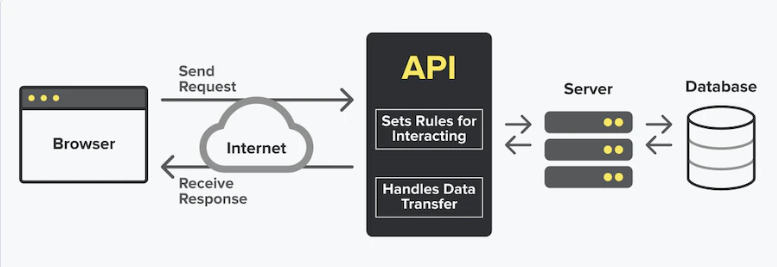
\includegraphics[width=0.8\columnwidth]{./images/front-end to database.png} 
  \label{fig_sim}
  \end{figure}
\subsection{The API integration in email notification feature}
When a user wants to use the email notification feature, the back-end of the Time Management Application will request the user's scheduler data from the database using the API. Once the data is retrieved, the back-end will then send the data to an external email application to generate a notification email, which will be sent to the user's specified email address. This process of data retrieval and communication between the back-end and external application is facilitated by the API integration.

\section{Benefits and Drawbacks} \label{sec:criteria}
Benefits:
\begin{itemize}
  \item The API integration enables seamless interaction between different components/features of the application.
  \item The API also handles data transfer of different language.
  \item API management enables users to track and monitor important metrics such as API usage, load, transaction logs, and historical data. 
\end{itemize}

Drawbacks
\begin{itemize}
  \item APIs can be a primary target for hackers. Once compromised, other systems become vulnerable.
\end{itemize}

\section{Conclusion}

In conclusion, API integration is critical for the efficient operation of a Time Management Application, allowing for seamless communication between different layers and features. The front-end and back-end API integration handles user input and display output, while the API integration in saving data enables users to save their data online or in the cloud. Finally, the API integration in the email notification feature facilitates the communication between the back-end and external email application. While there are benefits to API integration, such as improving application performance and tracking important metrics, there are also drawbacks to consider, such as the risk of being targeted by hackers. 

\begin{thebibliography}{1}
% Here are a few examples of different citations 
% Book
\bibitem{Lydia Pert} % Note the label in the curly brackets. Use the cite the source; e.g., \cite{kopka_latex}
Lydia Pert, \href{https://openvpn.net/blog/advantages-and-disadvantages-of-api-for-business/#:~:text=API%20Disadvantages&text=As%20a%20single%20point%20of,applications%20and%20systems%20become%20vulnerable.}{advantages and Disadvantages of API for Business}. [Accessed on: March.2, 2023]
\bibitem{Alex Trost}
Alex Trost, \href{https://snipcart.com/blog/integrating-apis-introduction}{A Beginner's Guide to APIs: How to Integrate and Use Them}. [Accessed on: March.2, 2023]
\bibitem{}
\href{https://www.mulesoft.com/resources/api/what-is-api-management#:~:text=API%20management%20is%20the%20process,create%20are%20consumable%20and%20secure.}{What is API management?}. [Accessed on: March.2, 2023]
\end{thebibliography}

% This is a hand-made bibliography. If you want to use a BibTeX file, you're on your own ;-)


\end{document}